\documentclass[11pt,a4paper]{article}
\usepackage[utf8]{inputenc}
\usepackage[T1]{fontenc}
\usepackage[margin=2.5cm]{geometry}
\usepackage{booktabs}
\usepackage{amsmath}
\usepackage{siunitx}
\usepackage{multirow}
\usepackage{float}
\usepackage[autostyle]{csquotes}
\usepackage[hidelinks]{hyperref}
\usepackage{graphicx}

\sisetup{detect-weight=true}

\title{\bfseries Marocco FL thesis --- week 26/10 update}
\author{}
\date{}

\begin{document}
\maketitle
\vspace{-3.2em}
\begin{center}
\emph{Client-Driven Local Work Assignment in Battery-Constrained Federated Learning}
\end{center}
\vspace{1em}

%======================================================================
\section*{Summary}

\begin{itemize}
  \item The ResNet-18 / CIFAR-100 campaign now has \textbf{three seeds}
        (2026, 42, 73): 14 labels $\times$ 3 $\beta$ $\times$ 3 seeds = 126 runs.
  \item \textbf{ESCS} was aligned with the authors' source code, and its other
        three variants (SP, MD, MP) were added (datasheet battery; the linear and
        Peukert worlds are running).
  \item Over the 9 pairs (3 $\beta$ $\times$ 3 seeds) against FedAvg ($B=128$),
        SAGE-smart \textbf{uses 35--44\,\% less energy in every pair}, depletes
        8 devices instead of 58, and is \textbf{+2.3 accuracy points} more
        accurate on average (better in 7--8 pairs out of 9). SAGE and all ESCS
        variants are 5--8 points below FedAvg.
  \item \textbf{Cumulative ablation} (Section~\ref{sec:cum}): starting from
        SAGE-smart with everything off and adding one component at a time, three
        steps make the difference: \textbf{staleness} (+5.5 points),
        \textbf{adaptive epochs} ($-774$~Wh, 24 depleted devices fewer) and the
        \textbf{small batch} (+9.1 points). Negotiation, SoC estimate and FedNova
        add nothing measurable, as in the leave-one-out of the 19/10 report.
  \item New runs record the \textbf{simulated time}. It shows that with adaptive
        epochs the 250 rounds last \textbf{11--12 hours instead of 25}, and that
        more than half of the energy saved by that step is idle consumption of the
        phones in the shorter run. The comparison at equal elapsed time is still
        to be done (Section~\ref{sec:time}).
\end{itemize}

%======================================================================
\section{What changed since the 19/10 report}

\begin{table}[H]
\centering
\small
\caption{Changes since the 19/10 report.}
\label{tab:changes}
\begin{tabular}{p{3.2cm}p{5.6cm}p{6.2cm}}
\toprule
item & now & note \\
\midrule
seeds & 2026, 42, 73 & 2026 reused: the code of the normal runs is unchanged and the runs are reproducible (checked bit for bit) \\
ESCS & aligned with the authors' source code (\texttt{escs\_sd/sp/md/mp.py}) & Section~\ref{sec:escs}; ESCS-SD seed 2026 rerun with the new code \\
ESCS variants & SD, SP, MD, MP; SP/MD/MP with the datasheet battery & linear and Peukert worlds for SP/MD/MP: running (54 runs) \\
cumulative ablation & 6 new steps, seed 2026, datasheet battery & Section~\ref{sec:cum} \\
simulated time & columns \texttt{round\_s}, \texttt{sim\_time\_s} in the CSV & logging only; present in the runs made after 27/10 (cumulative ablation, ESCS in the other worlds) \\
\bottomrule
\end{tabular}
\end{table}

%======================================================================
\section{ESCS: aligned with the authors' code}
\label{sec:escs}

The paper (Maciel et al.\ 2024) has no link to its code; the four source files
of the authors (Flower, TensorFlow) were compared line by line with our
implementation.

\paragraph{Already identical.} Resource filter (battery minus predicted
consumption $\geq 20\,\%$ and network quality $\geq 0.2$); system-based utility
$U_S=(w_b b + w_t(1-t)\,th + w_q q)^{1-\ell/\ell_{\max}}$; model-based utility
$U_M=(\ell/\ell_{\max})^{1-(w_b b + w_t(1-t)\,th + w_q q)}$ (the code resolves
an ambiguity of the formula printed in the paper the same way we had); time
penalty $th$ with the 95th percentile; all clients in round 1; $k=$ round$(N\,C)$
clients in the deterministic variants; probabilistic variants with no cap; static
network quality per client; data-weighted aggregation.

\paragraph{Changed to match their code.}
\begin{itemize}
  \item The loss used in the utility is the \textbf{training} loss reported by
        the selected clients (\texttt{fit\_res.metrics["loss"]}), not the
        evaluation loss. With 20\,\% of the clients evaluated per round, the
        evaluation loss was also on average 5 rounds old.
  \item SP/MP, when the draw selects nobody: the best round$(|\text{eligible}|\cdot C)$
        by utility. Last fallback (battery only): round$(n\,C)$ clients by loss.
\end{itemize}

\paragraph{Differences that remain (declared).}
\begin{itemize}
  \item \textbf{No transmission failures}: their simulator drops the update of a
        client whose per-round network quality is below the threshold. This is
        part of their environment; ours has no network failures for any
        algorithm, and adding them only to ESCS would not be a fair comparison.
  \item \textbf{Static network quality}, as in their code: clients with $q<0.2$
        never pass the filter after round 1 (13 / 22 / 22 clients out of 100 with
        seeds 2026 / 42 / 73).
  \item Global 20\,\% battery threshold, weights $1/3$, predicted consumption =
        drop of the client's last round, random tie-break; their
        $\infty/\infty=\text{NaN}$ for never-observed clients is not reproduced.
\end{itemize}

\paragraph{The probabilistic variants select many more clients.} With our
values most utilities are 0.8--0.9 and the draw has no cap: ESCS-SP and ESCS-MP
select about \textbf{46--47 clients per round} in rounds 2--50 (20 for SD/MD),
falling to 10--14 in the last 50 rounds as batteries run out. As in the paper,
they are the most energy-hungry variants.

%======================================================================
\section{Results with three seeds}
\label{sec:results}

\emph{Accuracy} is the mean over the last 20 rounds; \emph{depleted}: devices
that reached 0 (they never come back); $\pm$ is the standard deviation over the
three seeds.

\begin{table}[H]
\centering
\small
\caption{Main results per $\beta$ (mean $\pm$ std over 3 seeds) and mean over
the three $\beta$. SAGE ablation, ESCS and SAGE-smart with the datasheet battery;
FedAvg and SAGE (paper) in the linear world.}
\label{tab:main}
\begin{tabular}{lrrrr}
\toprule
& $\beta=0.1$ & $\beta=0.5$ & $\beta=1.0$ & \textbf{mean} \\
\midrule
\multicolumn{5}{l}{\textbf{Final accuracy} (\%)} \\
\quad FedAvg          & 49.9 $\pm$ 0.3 & 51.8 $\pm$ 0.9 & 52.9 $\pm$ 0.8 & 51.5 \\
\quad SAGE (paper)    & 43.6 $\pm$ 0.7 & 45.7 $\pm$ 1.8 & 47.0 $\pm$ 0.9 & 45.5 \\
\quad SAGE ablation   & 40.6 $\pm$ 1.5 & 45.2 $\pm$ 0.7 & 44.7 $\pm$ 3.1 & 43.5 \\
\quad ESCS-SD         & 42.8 $\pm$ 0.5 & 45.4 $\pm$ 1.3 & 45.9 $\pm$ 1.1 & 44.7 \\
\quad ESCS-MD         & 44.2 $\pm$ 0.7 & 47.8 $\pm$ 0.5 & 47.7 $\pm$ 1.8 & 46.6 \\
\quad ESCS-SP         & 42.1 $\pm$ 1.2 & 45.9 $\pm$ 0.5 & 47.0 $\pm$ 0.3 & 45.0 \\
\quad ESCS-MP         & 40.9 $\pm$ 0.5 & 45.2 $\pm$ 0.9 & 44.1 $\pm$ 1.8 & 43.4 \\
\quad SAGE-smart      & \textbf{50.2} $\pm$ 2.9 & \textbf{55.8} $\pm$ 1.7 & \textbf{55.5} $\pm$ 2.2 & \textbf{53.9} \\
\midrule
\multicolumn{5}{l}{\textbf{Energy drawn from the batteries} (Wh)} \\
\quad FedAvg          & 2151 $\pm$ 89  & 2036 $\pm$ 93  & 2004 $\pm$ 75 & 2064 \\
\quad SAGE (paper)    & 2187 $\pm$ 92  & 2046 $\pm$ 67  & 2094 $\pm$ 44 & 2109 \\
\quad SAGE ablation   & 1963 $\pm$ 102 & 1940 $\pm$ 75  & 1941 $\pm$ 43 & 1948 \\
\quad ESCS-SD         & 1944 $\pm$ 54  & 1982 $\pm$ 31  & 1944 $\pm$ 71 & 1956 \\
\quad ESCS-MD         & 2011 $\pm$ 34  & 2033 $\pm$ 37  & 1983 $\pm$ 48 & 2009 \\
\quad ESCS-SP         & 2209 $\pm$ 102 & 2218 $\pm$ 38  & 2181 $\pm$ 62 & 2203 \\
\quad ESCS-MP         & 2126 $\pm$ 70  & 2094 $\pm$ 186 & 1911 $\pm$ 23 & 2043 \\
\quad SAGE-smart      & \textbf{1313} $\pm$ 41 & \textbf{1206} $\pm$ 19 & \textbf{1195} $\pm$ 29 & \textbf{1238} \\
\midrule
\multicolumn{5}{l}{\textbf{Depleted devices} (of 100)} \\
\quad FedAvg          & 58.0 $\pm$ 1.7 & 58.0 $\pm$ 9.5 & 58.0 $\pm$ 13.1 & 58.0 \\
\quad SAGE (paper)    & 35.3 $\pm$ 3.8 & 34.0 $\pm$ 3.6 & 27.0 $\pm$ 7.0  & 32.1 \\
\quad SAGE ablation   & 31.0 $\pm$ 3.6 & 28.7 $\pm$ 4.2 & 27.0 $\pm$ 0.0  & 28.9 \\
\quad ESCS-SD         & 30.3 $\pm$ 2.3 & 31.3 $\pm$ 7.6 & 34.7 $\pm$ 2.9  & 32.1 \\
\quad ESCS-MD         & 34.0 $\pm$ 6.1 & 36.0 $\pm$ 7.0 & 32.7 $\pm$ 2.3  & 34.2 \\
\quad ESCS-SP         & 47.0 $\pm$ 2.6 & 45.0 $\pm$ 3.6 & 44.3 $\pm$ 5.8  & 45.4 \\
\quad ESCS-MP         & 43.7 $\pm$ 4.6 & 37.0 $\pm$ 2.6 & 42.3 $\pm$ 2.3  & 41.0 \\
\quad SAGE-smart      & \textbf{10.7} $\pm$ 1.2 & \textbf{7.7} $\pm$ 2.1 & \textbf{7.0} $\pm$ 1.0 & \textbf{8.4} \\
\bottomrule
\end{tabular}
\end{table}

\begin{table}[H]
\centering
\small
\caption{All labels, mean over the three $\beta$ (each $\beta$ averaged over 3
seeds). $<20\,\%$: devices that end below \SI{20}{\percent}, depleted included.
1st: round of the first depletion. $E_{40}$: energy spent to reach 40\,\%
accuracy (mean of 10 rounds).}
\label{tab:all}
\begin{tabular}{lrrrrrrrrr}
\toprule
& acc. & energy & train & idle & SoC & depleted & $<20\,\%$ & 1st & $E_{40}$ \\
& (\%) & (Wh) & (Wh) & (Wh) & (\%) & & & & (Wh) \\
\midrule
FedAvg                    & 51.5 & 2064 & 945 &  878 & 21.3 & 58.0 & 65.4 &  62 &  764 \\
FedProx                   & 51.3 & 2064 & 945 &  878 & 21.3 & 58.0 & 65.4 &  62 &  760 \\
\midrule
SAGE (paper, linear)      & 45.5 & 2109 & 833 & 1043 & 33.3 & 32.1 & 46.1 &  71 & 1182 \\
SAGE ablation (Peukert)   & 44.9 & 2011 & 761 & 1048 & 38.0 & 23.6 & 29.0 &  87 & 1068 \\
SAGE ablation (datasheet) & 43.5 & 1948 & 685 & 1074 & 36.9 & 28.9 & 34.7 &  80 & 1163 \\
\midrule
ESCS-SD (linear)          & 44.7 & 2042 & 840 &  964 & 34.5 & 31.1 & 45.4 &  72 & 1180 \\
ESCS-SD (Peukert)         & 45.1 & 1973 & 841 &  899 & 36.3 & 28.2 & 41.4 &  79 & 1084 \\
ESCS-SD (datasheet)       & 44.7 & 1956 & 810 &  917 & 34.6 & 32.1 & 44.6 &  67 & 1111 \\
ESCS-SP (datasheet)       & 45.0 & 2203 & 1090 & 823 & 29.8 & 45.4 & 56.8 &  45 & 1291 \\
ESCS-MD (datasheet)       & 46.6 & 2009 & 821 &  959 & 34.0 & 34.2 & 46.1 &  67 &  973 \\
ESCS-MP (datasheet)       & 43.4 & 2043 & 932 &  864 & 34.9 & 41.0 & 48.7 &  48 & 1333 \\
\midrule
SAGE-smart (linear)       & \textbf{54.1} & 1265 & 457 & 573 & 41.5 & 7.0 & 22.3 & 167 & 512 \\
SAGE-smart (Peukert)      & 54.0 & 1245 & 465 & 549 & 42.2 & \textbf{6.2} & \textbf{19.9} & 166 & 521 \\
SAGE-smart (datasheet)    & 53.9 & \textbf{1238} & 441 & 571 & \textbf{42.2} & 8.4 & 22.3 & 156 & \textbf{500} \\
\bottomrule
\end{tabular}
\end{table}

\begin{table}[H]
\centering
\small
\caption{Paired comparison with FedAvg on the same seed and $\beta$ (9 pairs).
One-sided sign test on 9 pairs: 7/9 $p=0.090$, 8/9 $p=0.020$, 9/9 $p=0.002$.}
\label{tab:paired}
\begin{tabular}{lrrr}
\toprule
& more accurate than FedAvg & $\Delta$ accuracy (points) & energy saved (min--max) \\
\midrule
FedProx                   & 1/9 & $-0.3 \pm 0.3$ & $0.0\,\%$ \\
SAGE (paper)              & 0/9 & $-6.1 \pm 1.3$ & $-2.3\,\%$ ($-7.7$ to $+2.2$) \\
SAGE ablation (datasheet) & 0/9 & $-8.0 \pm 2.0$ & $+5.4\,\%$ ($-3.6$ to $+9.7$) \\
ESCS-SD (datasheet)       & 0/9 & $-6.8 \pm 1.3$ & $+5.0\,\%$ ($-2.0$ to $+10.9$) \\
ESCS-MD (datasheet)       & 0/9 & $-5.0 \pm 1.7$ & $+2.5\,\%$ ($-4.1$ to $+8.9$) \\
ESCS-SP (datasheet)       & 0/9 & $-6.5 \pm 1.3$ & $-6.9\,\%$ ($-14.9$ to $-0.6$) \\
ESCS-MP (datasheet)       & 0/9 & $-8.1 \pm 1.8$ & $+0.9\,\%$ ($-16.1$ to $+8.3$) \\
SAGE-smart (linear)       & \textbf{8/9} & $+2.6 \pm 2.1$ & \textbf{+38.6\,\%} ($+35.2$ to $+42.3$) \\
SAGE-smart (Peukert)      & 7/9 & $+2.4 \pm 2.6$ & +39.6\,\% ($+36.3$ to $+41.7$) \\
SAGE-smart (datasheet)    & 7/9 & $+2.3 \pm 2.5$ & +40.0\,\% ($+36.0$ to $+43.9$) \\
\bottomrule
\end{tabular}
\end{table}

\begin{figure}[H]
\centering
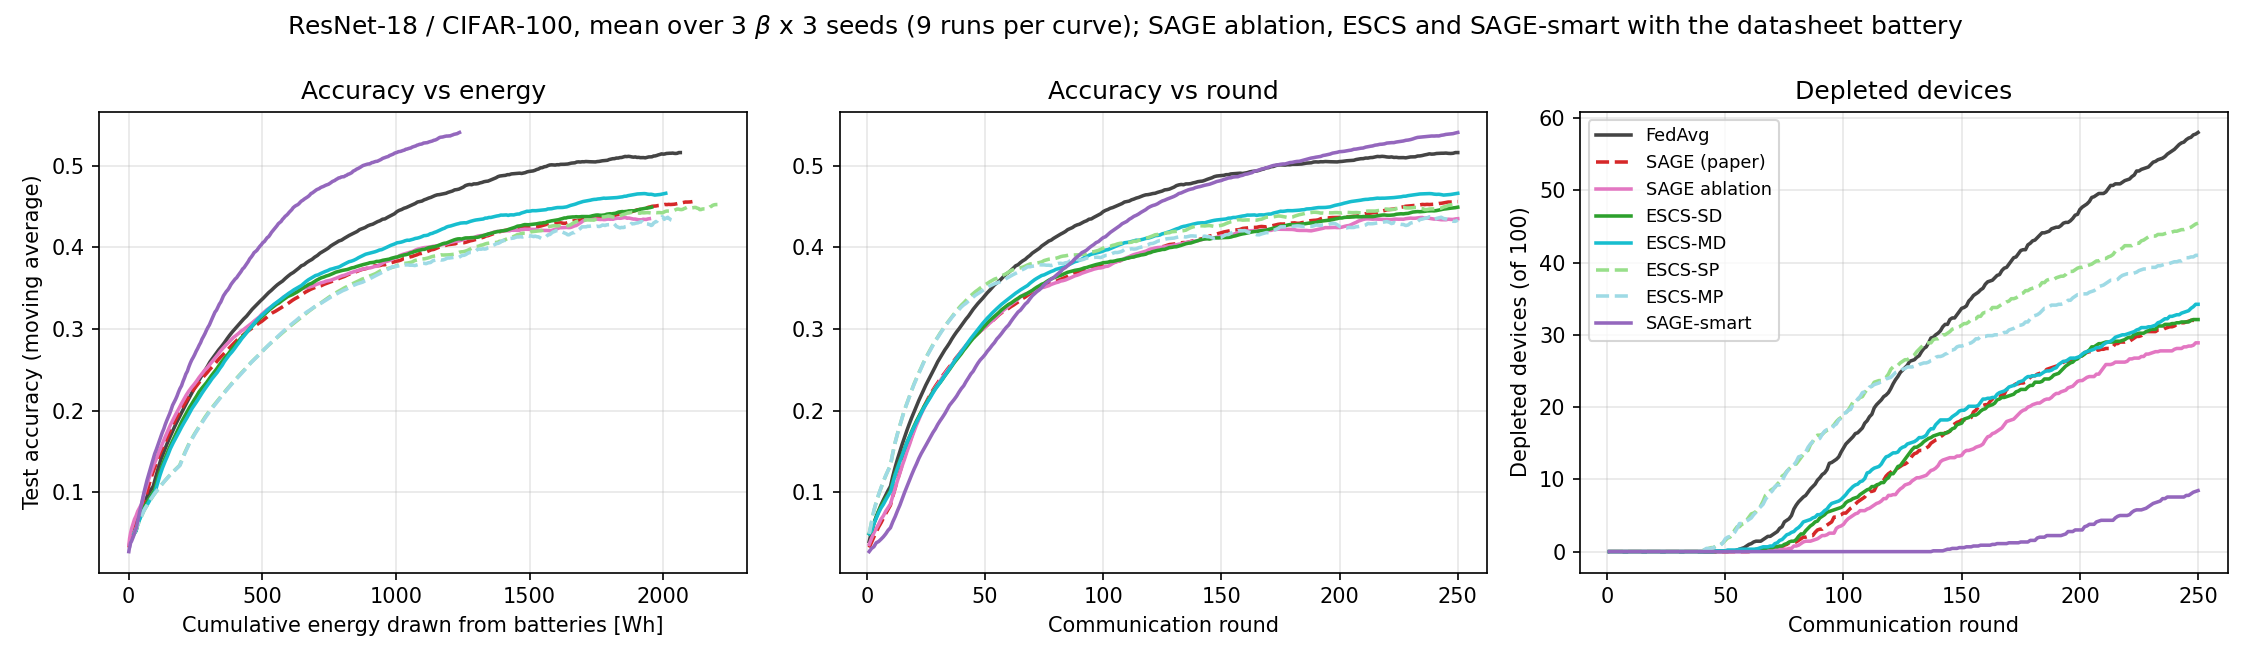
\includegraphics[width=\textwidth]{report13_figs/fig_main_3seeds.png}
\caption{Accuracy against energy, accuracy against rounds and depleted devices;
each curve is the mean of 9 runs (3 $\beta$ $\times$ 3 seeds). ESCS variants
shown separately.}
\label{fig:main}
\end{figure}

\paragraph{What the three seeds say.}
\begin{itemize}
  \item \textbf{Energy}: SAGE-smart saves 35--44\,\% against FedAvg in each of
        the 9 pairs, in all three battery worlds ($p=0.002$). It is the most
        robust result of the thesis so far (but see Section~\ref{sec:time}).
  \item \textbf{Batteries}: 2--12 depleted devices per run against 46--72 for
        FedAvg; the first depletion comes at round 156--167 instead of 62.
  \item \textbf{Accuracy}: equal to FedAvg at $\beta=0.1$ ($+0.0$ to $+0.6$
        points, 1--2 seeds out of 3), $+4.0$ to $+4.5$ points at $\beta=0.5$ and
        $+2.6$ to $+2.9$ at $\beta=1.0$ (3 seeds out of 3). Over the 9 pairs: 7/9
        with the datasheet battery ($p=0.09$), 8/9 with the linear one
        ($p=0.02$). SAGE-smart varies more from seed to seed (up to $\pm$2.9
        points) than FedAvg ($\pm$0.3--0.9). This comparison is against FedAvg at $B=128$;
        FedAvg at $B=16$ (one seed, 19/10 report) was 5.5 points above SAGE-smart.
  \item \textbf{ESCS}: all four variants are 5--8 points below FedAvg. MD is the
        best ($-5.0$). SP and MP use the most energy (SP: 7\,\% more than FedAvg)
        and deplete the most devices (41--45, the first already at round 45--48),
        as the paper reports for the probabilistic variants.
  \item \textbf{SAGE} (paper and ablation): 6--8 points below FedAvg, with half
        of its depletions.
  \item \textbf{Battery world}: for SAGE-smart the three batteries differ by
        0.2 accuracy points, 27~Wh and 2 depleted devices; for ESCS-SD by 0.4
        points. The battery model changes the results little; it matters for
        the reserve, where the datasheet battery drains faster (see the 19/10
        report).
\end{itemize}

%======================================================================
\section{Cumulative ablation}
\label{sec:cum}

Starting from SAGE-smart with all removable components off (step 0), one
component is added at a time, in the order of importance of the leave-one-out;
step 6 is the full SAGE-smart. Datasheet battery, seed 2026, three $\beta$.
Step 0 is close to the SAGE ablation but not identical: it keeps the client-side
reserve of SAGE-smart (a client that cannot afford the work withdraws) and the
state broadcast.

\begin{table}[H]
\centering
\small
\caption{Cumulative ablation: value of each step (seed 2026). References:
FedAvg (linear battery) and SAGE ablation (datasheet), same seed.}
\label{tab:cum}
\begin{tabular}{lrrrr}
\toprule
& $\beta=0.1$ & $\beta=0.5$ & $\beta=1.0$ & \textbf{mean} \\
\midrule
\multicolumn{5}{l}{\textbf{Final accuracy} (\%)} \\
\quad 0\ \ base ($E=5$, $B=128$, $a\cdot\text{SoC}+b\cdot D$) & 38.2 & 41.6 & 42.9 & 40.9 \\
\quad 1\ \ + staleness              & 44.2 & 47.7 & 47.3 & 46.4 \\
\quad 2\ \ + adaptive epochs        & 42.7 & 46.9 & 46.3 & 45.3 \\
\quad 3\ \ + small batch            & 51.2 & 55.0 & 57.1 & \textbf{54.4} \\
\quad 4\ \ + negotiation            & 49.2 & 54.7 & 56.5 & 53.5 \\
\quad 5\ \ + SoC estimate           & 48.5 & 54.8 & 56.4 & 53.2 \\
\quad 6\ \ + FedNova = SAGE-smart   & 49.2 & 54.3 & 53.1 & 52.2 \\
\quad \emph{FedAvg / SAGE ablation} & \emph{49.8 / 41.8} & \emph{51.0 / 45.9} & \emph{52.4 / 45.1} & \emph{51.1 / 44.3} \\
\midrule
\multicolumn{5}{l}{\textbf{Energy} (Wh)} \\
\quad 0 & 2010 & 2029 & 1983 & 2007 \\
\quad 1 & 2002 & 2100 & 1987 & 2030 \\
\quad 2 & 1268 & 1278 & 1221 & 1256 \\
\quad 3 & 1267 & 1217 & 1207 & \textbf{1230} \\
\quad 4 & 1295 & 1209 & 1207 & 1237 \\
\quad 5 & 1262 & 1223 & 1222 & 1236 \\
\quad 6 & 1330 & 1226 & 1228 & 1261 \\
\quad \emph{FedAvg / SAGE ablation} & \emph{2077 / 1875} & \emph{1956 / 2004} & \emph{1919 / 1989} & \emph{1984 / 1956} \\
\midrule
\multicolumn{5}{l}{\textbf{Depleted devices}} \\
\quad 0 & 32 & 36 & 35 & 34.3 \\
\quad 1 & 35 & 29 & 35 & 33.0 \\
\quad 2 & 12 &  7 &  8 &  9.0 \\
\quad 3 & 12 &  7 &  5 & \textbf{8.0} \\
\quad 4 & 11 &  8 &  7 &  8.7 \\
\quad 5 & 15 &  9 &  3 &  9.0 \\
\quad 6 & 10 &  6 &  8 & \textbf{8.0} \\
\quad \emph{FedAvg / SAGE ablation} & \emph{57 / 32} & \emph{69 / 24} & \emph{72 / 27} & \emph{66.0 / 27.7} \\
\midrule
\multicolumn{5}{l}{\textbf{Mean final SoC} (\%)} \\
\quad 0 & 40.4 & 34.5 & 39.0 & 38.0 \\
\quad 1 & 36.0 & 38.6 & 35.4 & 36.7 \\
\quad 2 & 36.2 & 40.5 & 39.3 & 38.7 \\
\quad 3 & 41.3 & 40.0 & 41.6 & \textbf{41.0} \\
\quad 4 & 39.9 & 38.8 & 40.0 & 39.6 \\
\quad 5 & 36.5 & 37.4 & 42.3 & 38.7 \\
\quad 6 & 40.9 & 38.6 & 37.5 & 39.0 \\
\quad \emph{FedAvg / SAGE ablation} & \emph{20.2 / 38.2} & \emph{13.6 / 36.4} & \emph{9.4 / 35.8} & \emph{14.4 / 36.8} \\
\bottomrule
\end{tabular}
\end{table}

\begin{table}[H]
\centering
\small
\caption{Increment brought by each step (mean over the three $\beta$) and
simulated duration of the 250 rounds. The time is not recorded in the full
SAGE-smart run (made before the column existed).}
\label{tab:cum_delta}
\begin{tabular}{lrrrrrr}
\toprule
step & $\Delta$ acc. & $\Delta$ energy & $\Delta$ SoC & $\Delta$ depleted & simulated time & mean round \\
& (points) & (Wh) & (points) & & (h) & (s) \\
\midrule
0 base                &        &       &        &         & 25.5 & 367 \\
1 + staleness         & $+5.5$ & $+22$ & $-1.3$ & $-1.3$  & 25.9 & 373 \\
2 + adaptive epochs   & $-1.1$ & $\mathbf{-774}$ & $+2.0$ & $\mathbf{-24.0}$ & \textbf{11.6} & 167 \\
3 + small batch       & $\mathbf{+9.1}$ & $-25$ & $+2.3$ & $-1.0$ & 11.2 & 162 \\
4 + negotiation       & $-1.0$ & $+7$  & $-1.4$ & $+0.7$  & 11.3 & 163 \\
5 + SoC estimate      & $-0.2$ & $-1$  & $-0.8$ & $+0.3$  & 11.3 & 162 \\
6 + FedNova           & $-1.0$ & $+26$ & $+0.3$ & $-1.0$  & --- & --- \\
\bottomrule
\end{tabular}
\end{table}

\begin{figure}[H]
\centering
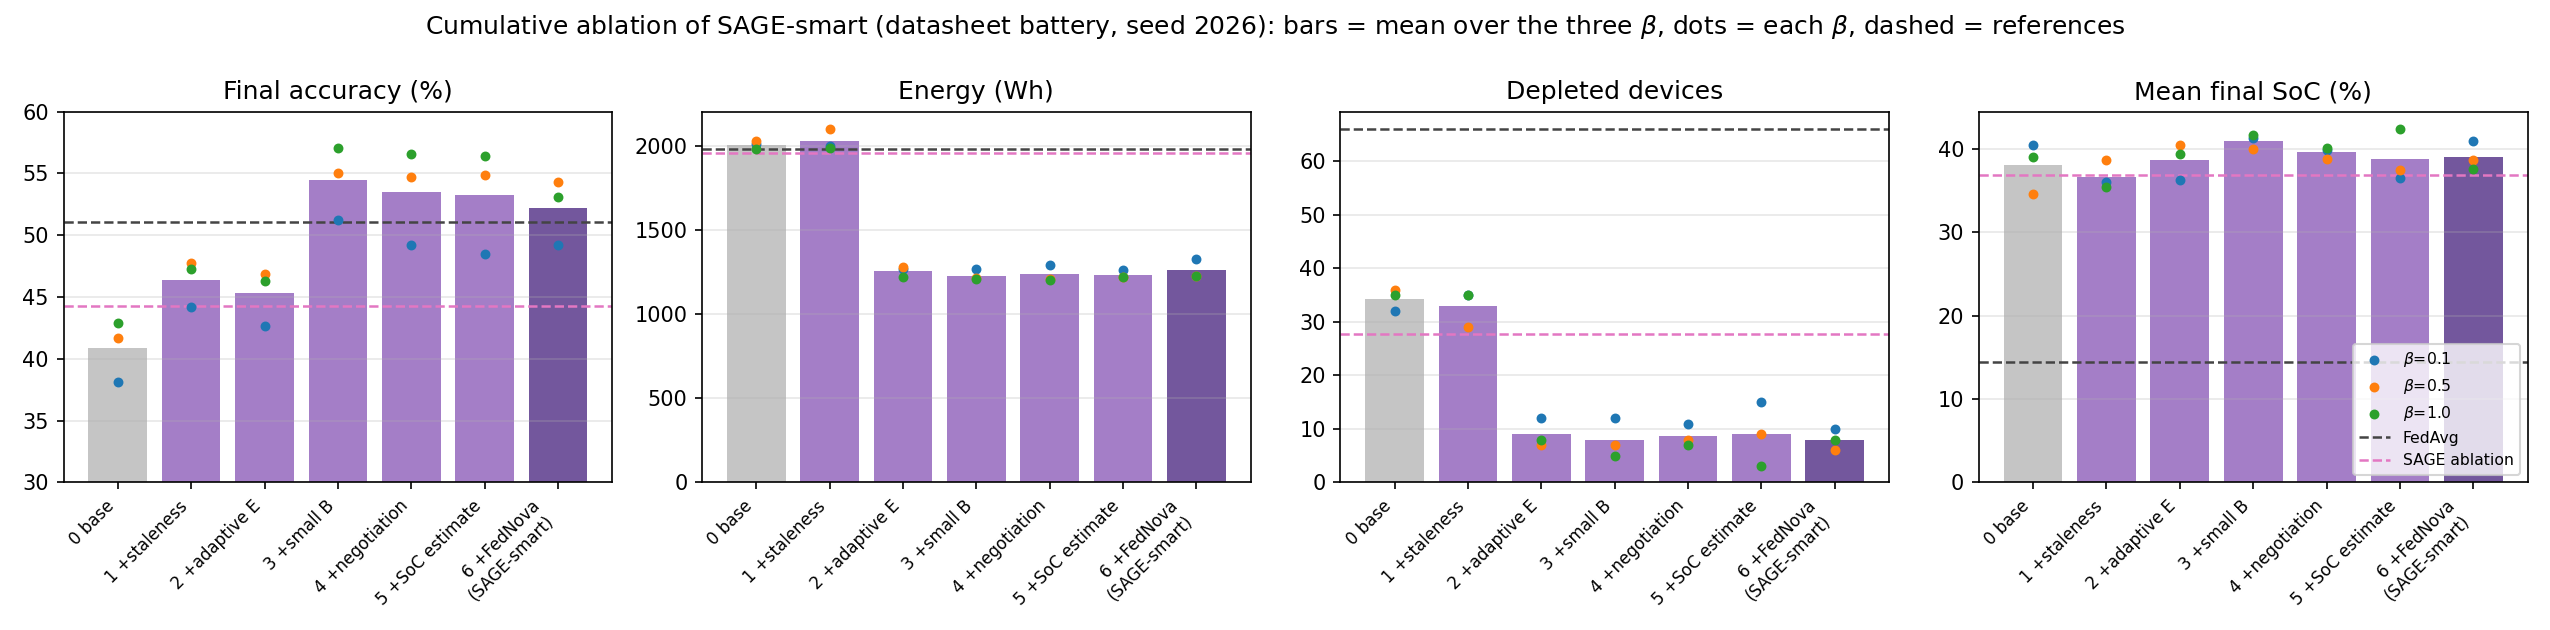
\includegraphics[width=\textwidth]{report13_figs/fig_cumulative_ablation.png}
\caption{Cumulative ablation: bars = mean over the three $\beta$, dots = each
$\beta$, dashed lines = FedAvg and SAGE ablation (seed 2026).}
\label{fig:cum}
\end{figure}

\paragraph{Reading the steps.}
\begin{itemize}
  \item \textbf{Staleness} (+5.5 points, no energy cost): without it the score
        keeps choosing the same clients; with it participation is spread over
        all clients and the model sees more data.
  \item \textbf{Adaptive epochs} ($-774$~Wh, $-38\,\%$; 24 depleted devices
        fewer; $-1.1$ points): the clients train 2.3--2.6 epochs instead of 5,
        bounded by the deadline. It is the engine of the energy saving and of the
        battery protection, as in the leave-one-out ($-791$~Wh, 23 devices).
  \item \textbf{Small batch} (+9.1 points, energy unchanged): with ResNet-18 the
        fixed cost per batch is negligible, so $B=16$--32 gives more SGD steps
        for the same energy. It is what brings SAGE-smart above FedAvg ($B=128$):
        at step 2 it is 6 points below.
  \item \textbf{Negotiation, SoC estimate, FedNova}: within $\pm1$ point,
        $\pm$\SI{26}{\watt\hour} and $\pm1$ device, i.e.\ within the noise of one
        seed (SAGE-smart varies by $\pm$2--3 points across seeds). Without the
        negotiation, 9--58 clients per run download the model and then withdraw;
        with it they refuse instead (3--100 refusals per run), at about the same
        energy.
  \item \textbf{Step 3 is as good as the full method} (54.4\,\%, \SI{1230}{\watt\hour},
        8 depleted devices) with three components fewer.
  \item \textbf{Consistency check}: step 5 (everything except FedNova) has
        exactly the configuration of the ``no FedNova'' run of the leave-one-out,
        and gives the same energy, SoC and depleted devices to the last digit.
\end{itemize}

%======================================================================
\section{A caveat from the simulated time}
\label{sec:time}

The new time column shows that the 250 rounds do not last the same time for all
methods. With $E=5$ and $B=128$ (steps 0--1) a round lasts 360--380~s, because
it waits for the slowest client (250 rounds $\approx$ 25 hours; FedAvg, which
does the same work, should be similar). With adaptive epochs the deadline caps
the round at about 160--170~s (250 rounds $\approx$ 11--12 hours).

This changes the reading of the energy saving. Step 2 saves
\SI{322}{\watt\hour} of training energy and \SI{482}{\watt\hour} of
\textbf{idle consumption} (communication grows by \SI{28}{\watt\hour}, because
more devices stay alive and are selected): the phones live through a run that
is 14 hours shorter. Against FedAvg, idle is about 37\,\% of the energy saved by SAGE-smart
(\SI{307}{} of \SI{826}{\watt\hour}). The same holds for the batteries: a
shorter run means fewer hours of drain (and fewer recharges).

All the comparisons so far are at \textbf{equal number of rounds}. At
\textbf{equal elapsed time}, SAGE-smart would run about twice as many rounds as
FedAvg: its accuracy would rise further, while its energy and battery advantage
would shrink. Both readings are legitimate, but the thesis has to state which
one it uses; the energy-versus-time figure (postponed) is what answers this.
It needs the time column, which the runs of the three-seed campaign do not
have.

%======================================================================
\section{Limits}

\begin{itemize}
  \item \textbf{FedAvg at $B=16$} has one seed only (it was 5.5 points above
        SAGE-smart at seed 2026). The accuracy comparison with three seeds is
        against FedAvg at $B=128$.
  \item \textbf{Equal rounds, not equal time} (Section~\ref{sec:time}).
  \item \textbf{ESCS}: no transmission failures, and 13--22 clients per seed are
        never selected because the network quality is static (as in the
        authors' code). SP/MD/MP in the linear and Peukert worlds are still
        running.
  \item \textbf{Cumulative ablation on one seed}: the steps of 5--9 points and
        of 700~Wh are clear; those of $\pm1$ point are not distinguishable.
  \item \textbf{Not converged}: SAGE-smart is still rising at round 250.
  \item \textbf{Depletion is permanent} (a device at 0 never recharges).
\end{itemize}

%======================================================================
\section{Next steps}

\begin{enumerate}
  \item \textbf{Energy against elapsed time}: rerun the main labels with the time
        column (seed 2026: the runs are reproducible, so the results are the same
        plus the time) and compare the methods at equal time.
  \item \textbf{FedAvg at $B=16$ with seeds 42 and 73} (6 runs).
  \item \textbf{ESCS SP/MD/MP in the linear and Peukert worlds}: running.
  \item \textbf{Which SAGE-smart to present}: the full method or the simpler
        step 3 (staleness + adaptive epochs + small batch), which is as good.
        Negotiation and SoC estimate could be kept as safety mechanisms and
        shown in a scenario where they matter (no broadcast, pauses between
        rounds, low batteries).
  \item \textbf{Battery-model figure}: why the Peukert and datasheet models are
        preferable to the linear one (voltage drop and error near the reserve).
  \item Pause of 10 minutes between rounds: to be confirmed.
\end{enumerate}

%======================================================================
\section*{References}

\begin{itemize}
  \item F.~Maciel et al., ``Federated learning energy saving through client
        selection'' (ESCS), Pervasive and Mobile Computing 103 (2024) 101948;
        source code of the four variants provided by the authors.
  \item M.~Savoia et al., ``SAGE: Sustainable and green energy-aware client
        selection for federated learning'', Applied Energy 410 (2026) 127568.
  \item J.~Wang et al., ``Tackling the Objective Inconsistency Problem in
        Heterogeneous Federated Optimization'' (FedNova), NeurIPS 2020.
  \item K.~He, X.~Zhang, S.~Ren, J.~Sun, ``Deep Residual Learning for Image
        Recognition'', CVPR 2016.
  \item Other references (phones, 4G, recharge, battery): see the 12/10 and
        19/10 reports.
\end{itemize}

\end{document}
